\documentclass[runningheads]{llncs}
\usepackage{graphicx}
\usepackage{tabularx}
\usepackage{amsmath}
\usepackage{multirow}
\newcommand{\code}[1]{\texttt{#1}}
\usepackage{xcolor}
\usepackage{fancyvrb}
\usepackage{listings}
\lstloadlanguages{Python}
\lstset{
  language=Python,
  basicstyle=\scriptsize\sffamily,
  numberstyle=\color{gray},
  stringstyle=\color[HTML]{933797},
  commentstyle=\color[HTML]{228B22}\sffamily,
  emph={[2]from,import,pass,return}, emphstyle={[2]\color[HTML]{DD52F0}},
  emph={[3]range}, emphstyle={[3]\color[HTML]{D17032}},
  emph={[4]for,in,def}, emphstyle={[4]\color{blue}},
  showstringspaces=false,
  breaklines=true,
  prebreak=\mbox{{\color{gray}\tiny$\searrow$}},
  numbers=left,
  xleftmargin=15pt
}
\setlength{\intextsep}{10pt plus 2pt minus 2pt}

%%%%% START DOCUMENT %%%%%
\begin{document}

\title{COMP 472 Project 2 \\ Naive Bayes Classifier}

\author{Matteo Esposito\inst{1} \and
Matthew Liu\inst{2} \and
Kabir Soni\inst{3}}

\authorrunning{M. Esposito et al.}

\institute{40024121 \email{matteoesposito97@gmail.com} \and
40029238 \email{matthew.jx.liu@gmail.com} \and
40033019 \email{kabirsoni524@gmail.com}}

\maketitle   

\section{Introduction \& Technical Details}

This project was developed using python 3.7.4 64-bit.

\subsection{Files}

The file structure of our project is as follows:

\begin{table}
    \centering
    \caption{Files in project 1}\label{tab0}
    \begin{tabularx}{\textwidth}{|l|l|X|}
        \hline
        \textbf{Directory} & \textbf{Filename} & \textbf{Usage} \\ \hline
        \verb|out/| & * & Trace and evaluation files for each run. \\ \hline
        \verb|out_BYOM/| & * & Trace and evaluation files for each BYOM run. \\ \hline
        \verb|src/| & \verb|utils.py| & Helper functions for I/O and input parsing. \\ \hline
                    & \verb|NBClassifier.py| & Naive Bayes Classifier class. A collection of methods used to implement Naive Bayes Classification. \\ \hline
                    & \verb|Ngram.py| & Ngram class, used in all classifications. \\ \hline
                    & \verb|BYOM.py| & Personalized model class. \\ \hline
                    & \verb|main.py| & Reading training set, training classifier, predicting languages on test set and writing out results. \\ \hline
    \end{tabularx}
\end{table}

\subsection{Packages}

We used a total of 7 packages in our project, 5 existing, along with our 2 internal packages (board and node). 

\begin{enumerate}
    \item Existing 
    \begin{itemize}
        \item \verb|shutil| and \verb|os|: Folder and file management in the creation and deletion of output folders for our search and solution files. 
        \item \verb|math|: Calculating log base 10 probabilities as part of the score function of each tweet.
        \item \verb|copy|: Used to create deep copies in the initialization of ngrams in the NBClassifier class.
        \item \verb|decimal.Decimal|: Used to format the probability output for the trace file.
        \item \verb|string|: Used to populate vocabulary 1 and 2 with ascii characters.
    \end{itemize}
    \item Internal
    \begin{itemize}
        \item \verb|NBClassifier|: Class that is used to represent the classifier, which takes a vocabulary selection, ngram size, delta/smoothing value and train/test file links.
        \item \verb|Ngram|: Class used to represent the Ngram used in the NBClassifier class. 
    \end{itemize}
\end{enumerate}

\subsection{NBClassifier and Ngram Classes}

The \textbf{Ngram} class will be used in the NBClassifier class. It allows for a concise way to store a language, count/frequency table, probability table and language probability. This class stores the probability calculation, smoothing and language probability methods which are called in the train method of NBClassifier.

\medskip

The \textbf{NBClassifier} class will have as main attributes a language, count table, probability table and size $(n)$, which will all be stored in a size-$n$ Ngram. It will also hold a language probability. It is from the NBClassifier object in \code{main.py} that we will call the train and predict methods.

\medskip

\underline{Note on vocabulary creation:} Vocabularies 0 and 1 are generated by combining ascii character sets from the \code{string} library. Vocabulary 3 is created by only considering the words in the training set for which \code{is\_alpha()} returns \code{True}. All the unseen words in the test set are then treated as a single group.

\newpage

\section{Dataset Impact \& Analysis}

In our exploratory data analysis we assess 2 characteristics of the test sets, namely tweet length and language frequency.

\subsection{Tweet Length}

Rounding down all tweets with length larger than 150 charaters down to 150 (as they make up less than 0.5\% of the observations), we get the following capped tweet length distribution curves for the provided and demo test sets of tweets.

\begin{figure}
    \begin{center}
        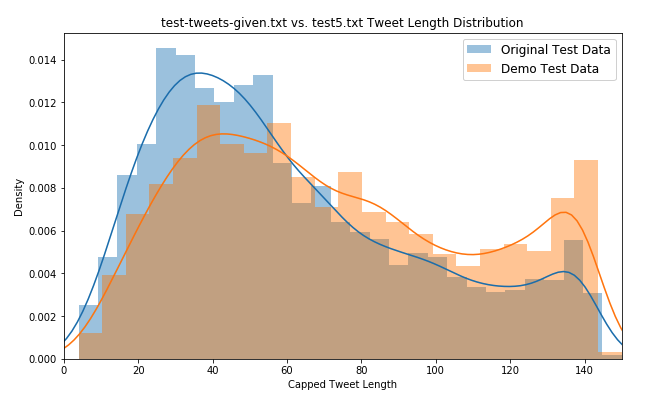
\includegraphics[width=12.5cm]{images/tlendist.png}
    \end{center}
\end{figure}

The main observation we can notice from the overlayed distribution plots is that the demo test set contains a greater proportion of large tweets (tweets with length over $\sim 70$ characters). The effect this could have on the accuracy of our classifications is that we are introducing a larger amount of unigrams, bigrams and trigrams from the tweet being assessed by the classifier and therefore introducing the potential for a greater amount of incorrectly labelled character patterns.

\subsection{Language Frequency}

Generating a frequency table of the languages in the provided test dataset we observe the following:

\begin{verbatim}
orig_test.lang.value_counts()

    es    3926
    pt    2020
    en     505
    eu     376
    ca      75
    gl       1

\end{verbatim}

We notice that there is a single observation in the 'gl' class. This will have an effect on our precision, recall and f1 values. In the case where we do not correctly classify that observation into the 'g1' class, our true positive value for the gl class will be 0, making precision and recall also 0 and yielding an f1 value of $0/0$ (which we set to 0 in this case).

\medskip

Generating a frequency table of the languages in the demo test dataset we observe the following:

\begin{verbatim}
demo_test.lang.value_counts()

    es    4572
    ca    1387
    gl     504
    en     483
    pt      96

\end{verbatim}

We notice that there are no observation in the 'eu' class. Every classification of a test tweet into the 'eu' class will result in a direct increase in the number of false positives, affecting our validation metrics negatively (decreasing precision and f1).

\section{Our Model (BYOM)}

\textcolor{red}{Kabir}

\newpage
\section{Result \& Experiment Analysis}

\subsection{Initial Test Set Results and Analysis}

\subsubsection{Model 1 ($V=0, n=1, \delta=0$): }
The first model had an accuracy of 0.686, a macro F1 of 0.461 and a weighted F1 of 0.653 on the pre-demo test set. The per-class metrics are shown in Figure~\ref{fig:pre_demo_0_1_0}. \\

\begin{figure}
    \begin{center}
        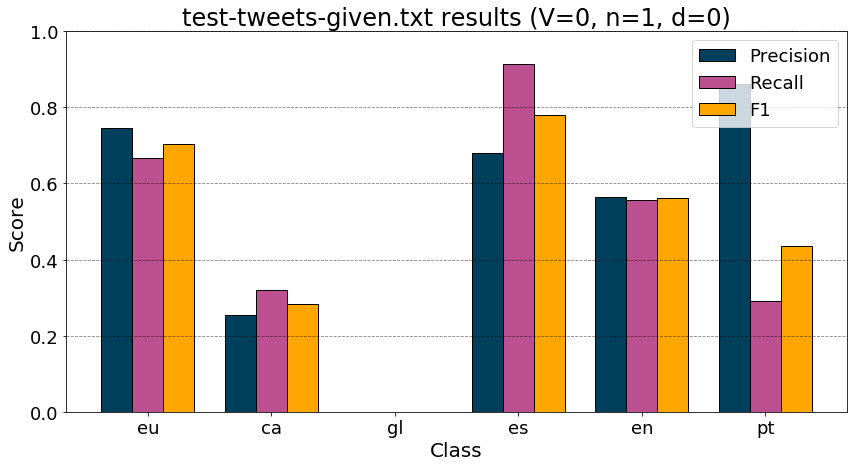
\includegraphics[width=12.5cm]{images/test_tweets_given_results_0_1_0.png}
        \caption{Metrics on original test set, $V=0, n=1, \delta=0$}
        \label{fig:pre_demo_0_1_0}
    \end{center}
\end{figure}

Out of all models, Model 1 performs the worst across all three global metrics on the original pre-demo test set. This is most likely due to the model's simplicity (only using unigrams with no smoothing). \\

The per-class metrics indicate that this first model is exhibits the highest precision for Portuguese tweets and the highest recall for Spanish tweets (see Appendix A Table~\ref{tab:pre_demo_confusion_0_1_0} for a more detailed confusion matrix). Although these results are promising, the other models tested performed at least as well or better than model 1 for these languages. \\

\begin{table}
	\centering
	\caption{Cross tabulation of predictions, $V=0, n=1, \delta=0$}
	\label{tab:pre_demo_confusion_0_1_0}
	\begin{tabular}{|c|c|c|c|c|c|c|c|} \hline
		& & \multicolumn{6}{c|}{Predicted} \\ \hline
		& &  ca &   en &    es &   eu &  gl &   pt \\ \hline
		\multirow{6}{*}{Actual} & ca   &  24 &    3 &    44 &    1 &   1 &    2 \\
		& en   &   7 &  287 &   205 &   11 &   0 &    6 \\
		& es   &  44 &  140 &  3635 &   63 &   3 &   88 \\
		& eu   &   3 &   16 &   107 &  253 &   0 &    1 \\
		& gl   &   0 &    0 &     1 &    0 &   0 &    0 \\
		& pt   &  16 &   62 &  1365 &   11 &   1 &  600 \\ \hline
	\end{tabular}
\end{table}

When looking at weaknesses, model 1 performed particularly poorly on all 3 metrics for Catalan tweets. This is perhaps surprising given the language's resemblance to Spanish and Portuguese, but this is likely due to the low proportion of Catalan language tweets in the test set. In fact, when looking at Table~\ref{tab:pre_demo_confusion_0_1_0}, we see that the model over-predicts the number of Catalan tweets, with 70 false positives and only 24 true positives. It also miss-classified many Catalan tweets as Spanish. \\

Finally, because of the test set consisted of only a single Galician, all metrics are 0 (we will ignore Galician tweets in our analysis because of this).

\subsubsection{Model 2 ($V=1, n=2, \delta=0.5$): }
The second model had an accuracy of 0.848, a macro F1 of 0.622 and a weighted F1 of 0.858 on the pre-demo test set. The per-class metrics are shown in Figure~\ref{fig:pre_demo_1_2_0.5}.

\begin{figure}
    \begin{center}
        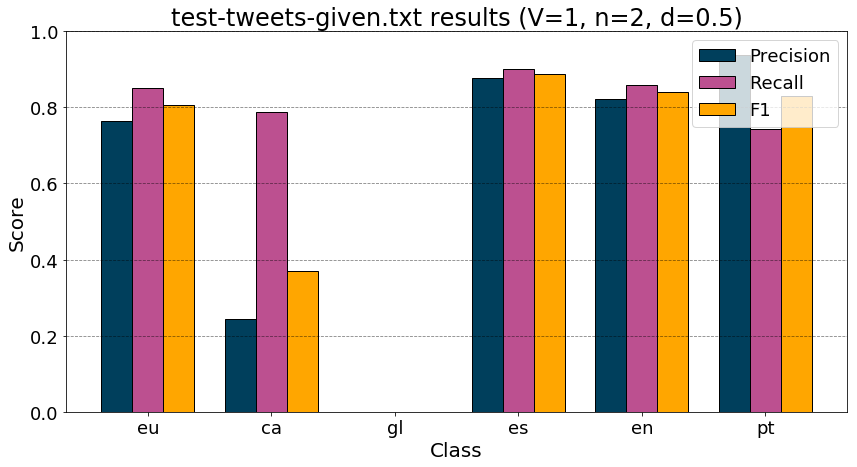
\includegraphics[width=12.5cm]{images/test_tweets_given_results_1_2_0.5.png}
        \caption{Metrics on original test set, $V=1, n=2, \delta=0.5$}
        \label{fig:pre_demo_1_2_0.5}
    \end{center}
\end{figure}

We see a significant improvement on overall accuracy for this model compared to the first (from 0.653 to 0.848). While the macro F1 measure is still relatively low, the more representative weighted F1 measure is much higher than the previous model. \\

When looking at the per-class metrics graph, we can see that all the problems of the first model were fixed, with all metrics close to or above 0.80. The only exception is the Catalan class. More specifically, the recall has improved significantly, but the other metrics are still poor. \\

Consulting Table~\ref{tab:pre_demo_confusion_1_2_0.5} reveals that model 2 still over-predicts the number of Catalan language tweets (confounding them with Spanish or Portuguese), which would explain the low precision. However, the sheer number of Catalan predictions (243) is able to raise the recall to close to 0.8. \\

\begin{table}
	\centering
	\caption{Cross tabulation of predictions, $V=1, n=2, \delta=0.5$}
	\label{tab:pre_demo_confusion_1_2_0.5}
	\begin{tabular}{|c|c|c|c|c|c|c|c|} \hline
		& & \multicolumn{6}{c|}{Predicted} \\ \hline
		& &   ca &   en &    es &   eu &  gl &    pt \\ \hline
		\multirow{6}{*}{Actual} & ca   &   59 &    1 &    14 &    0 &   0 &     1 \\
		& en   &    8 &  443 &    50 &    7 &   0 &     8 \\
		& es   &  110 &   66 &  3584 &   84 &  41 &    88 \\
		& eu   &    5 &    6 &    41 &  323 &   0 &     5 \\
		& gl   &    0 &    0 &     0 &    0 &   0 &     1 \\
		& pt   &   61 &   23 &   397 &    8 &  38 &  1528 \\ \hline
	\end{tabular}
\end{table}

Overall, the use of bigrams over unigrams and the addition of smoothing improves the model by a significant margin on all fronts.

\subsubsection{Model 3 ($V=1, n=3, \delta=1$): }
The third model had an accuracy of 0.877, a macro F1 of 0.664 and a weighted F1 of 0.873 on the pre-demo test set. The per-class metrics are shown in Figure~\ref{fig:pre_demo_1_3_1}. \\

\begin{figure}
    \begin{center}
        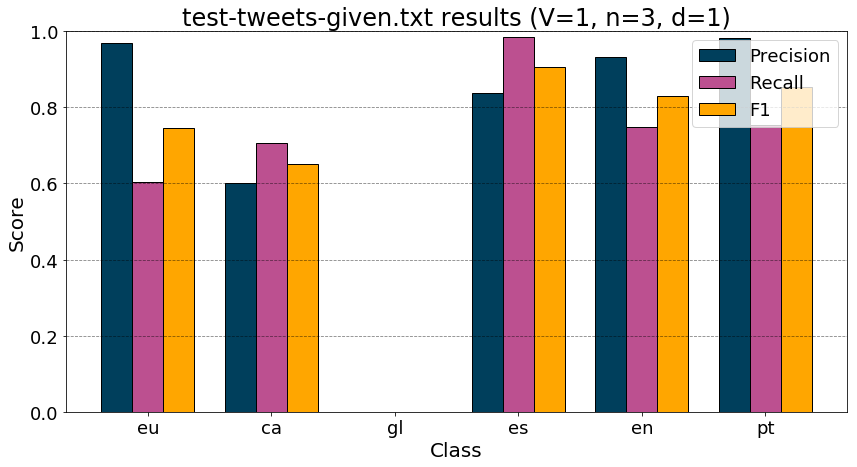
\includegraphics[width=12.5cm]{images/test_tweets_given_results_1_3_1.png}
        \caption{Metrics on original test set, $V=1, n=3, \delta=1$}
        \label{fig:pre_demo_1_3_1}
    \end{center}
\end{figure}

The overall accuracy and F1 metrics have improved yet again with a more complex model (using trigrams). This time, the precision also increased substantially for the Catalan class, with the recall dropping slightly. \\

The confusion matrix shown in Table~\ref{tab:pre_demo_confusion_1_3_1} shows that the model no longer seems to over-predict Catalan tweets as it used to. This however, is balanced out by an increase in predictions for Spanish (mirrored by the recall metric nearly reaching 1 for that class). This increase led in-turn to more false negatives for both the Basque and English language (with the former being a closely related language to Spanish).

\begin{table}
	\centering
	\caption{Cross tabulation of predictions, $V=1, n=3, \delta=1$}
	\label{tab:pre_demo_confusion_1_3_1}
	\begin{tabular}{|c|c|c|c|c|c|c|c|} \hline
		& & \multicolumn{6}{c|}{Predicted} \\ \hline
		& &  ca &   en &    es &   eu &  gl &    pt \\ \hline
		\multirow{6}{*}{Actual} & ca   &  53 &    1 &    21 &    0 &   0 &     0 \\
		& en   &   4 &  386 &   121 &    1 &   0 &     4 \\
		& es   &  10 &   15 &  3918 &    6 &   1 &    23 \\
		& eu   &   5 &    4 &   140 &  230 &   0 &     1 \\
		& gl   &   0 &    0 &     1 &    0 &   0 &     0 \\
		& pt   &  16 &    8 &   480 &    0 &   1 &  1550 \\ \hline
	\end{tabular}
\end{table}



\subsubsection{Model 4 ($V=2, n=2, \delta=0.3$): }
The fourth and final model had an accuracy of 0.88, a macro F1 of 0.651 and a weighted F1 of 0.884 on the pre-demo test set. The per-class metrics are shown in Figure~\ref{fig:pre_demo_2_2_0.3}. \\

\begin{figure}
    \begin{center}
        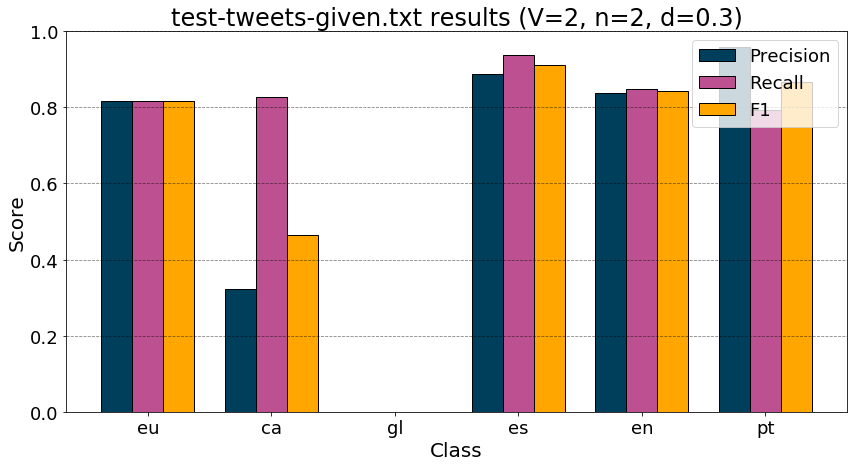
\includegraphics[width=12.5cm]{images/test_tweets_given_results_2_2_0.3.png}
        \caption{Metrics on original test set, $V=2, n=2, \delta=0.3$}
        \label{fig:pre_demo_2_2_0.3}
    \end{center}
\end{figure}

Once again the global metrics have increased across the board, but only marginally so when compared to model 3. It is undeniable that increasing the length to trigrams had a desirable effect on the model, as it was the only classifier that achieved a precision greater than 0.4 for Catalan tweets on the original test set, and consequently the only trigram model. While the results for the Catalan class regressed to the level of the second model, the F1 metrics for the other classes all improved.

\begin{table}
	\centering
	\caption{Cross tabulation of predictions, $V=2, n=2, \delta=0.3$}
	\label{tab:pre_demo_confusion_2_2_0.3}
	\begin{tabular}{|c|c|c|c|c|c|c|c|} \hline
		& & \multicolumn{6}{c|}{Predicted} \\ \hline
		& &  ca &   en &    es &   eu &  gl &    pt \\ \hline
		\multirow{6}{*}{Actual} & ca   &  62 &    1 &    12 &    0 &   0 &     0 \\
		& en   &   9 &  438 &    60 &    7 &   0 &     2 \\
		& es   &  70 &   55 &  3721 &   57 &  11 &    59 \\
		& eu   &   4 &    8 &    51 &  311 &   0 &     6 \\
		& gl   &   0 &    0 &     0 &    0 &   0 &     1 \\
		& pt   &  47 &   20 &   340 &    6 &  14 &  1628 \\ \hline
	\end{tabular}
\end{table}

We can probably assume that the increased vocabulary aided the model on a global level, while the use of bigrams may have hindered the classifier for the Catalan class. Overall, this final model performs the best when looking at the metrics.

\begin{figure}
    \begin{center}
        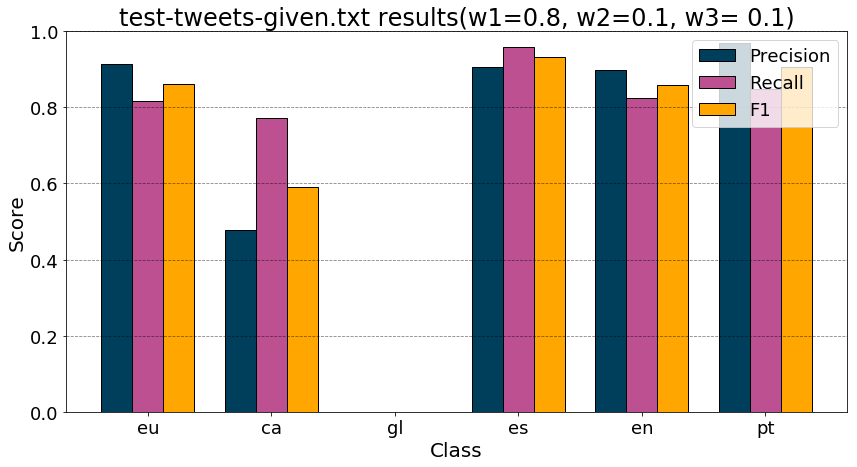
\includegraphics[width=12.5cm]{images/test_tweets_given_results_BYOM.png}
        \caption{Metrics on original test set, BYOM $w_1=0.8$, $w_2=0.1$, $w_3=0.1$}
        \label{fig:pre_demo_BYOM}
    \end{center}
\end{figure}

\newpage

\subsection{Demo Test Set Results and Analysis}

\subsubsection{Model 1 ($V=0, n=1, \delta=0$): }
The first model had an accuracy of 0.702, a macro F1 of 0.334 and a weighted F1 of 0.662 on the demo test set. The per-class metrics are shown in Figure~\ref{fig:demo_0_1_0}. \\

\begin{figure}
    \begin{center}
        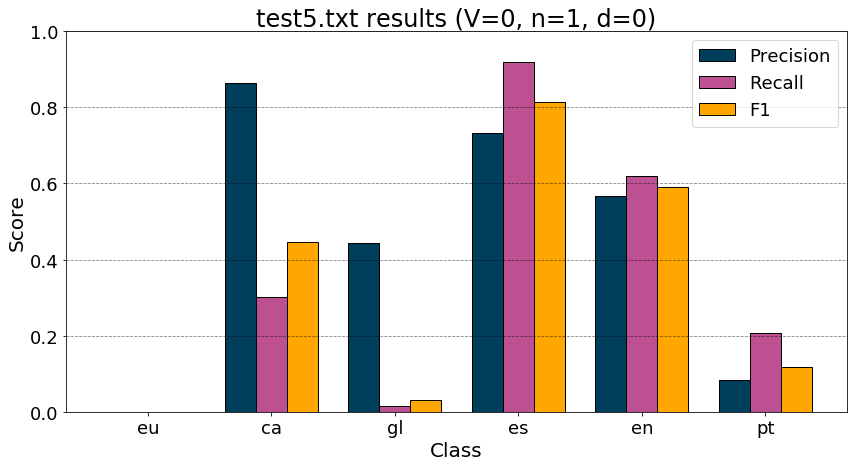
\includegraphics[width=12.5cm]{images/test5_results_0_1_0.png}
        \caption{Metrics on demo test set, $V=0, n=1, \delta=0$}
        \label{fig:demo_0_1_0}
    \end{center}
\end{figure}

Once again, model 1 performs the worst out of all models when testing on the demo test set. This is again most likely due to its simplicity and the absence of smoothing. When looking at the per-class charts, we can see that the model now performs most poorly on the Portuguese tweets. This makes sense when considering the low instance of the class in the test set. In fact, because of this low proportion, the classifier seems to over-predict for said class (see Table~\ref{tab:demo_confusion_0_1_0}), with most of the false positives falling in Spanish. \\

\begin{table}
	\centering
	\caption{Cross tabulation of predictions, $V=0, n=1, \delta=0$}
	\label{tab:demo_confusion_0_1_0}
	\begin{tabular}{|c|c|c|c|c|c|c|c|} \hline
        & & \multicolumn{6}{c|}{Predicted} \\ \hline
		& &    ca &   en &    es &  eu &   gl &   pt \\ \hline
		\multirow{6}{*}{Actual} & ca   &  418 &   52 &   868 &   5 &   5 &   43 \\
		& en   &    7 &  299 &   171 &   2 &   0 &    4 \\
		& es   &   51 &  164 &  4217 &  20 &   5 &  132 \\
		& gl   &    7 &    8 &   441 &   1 &   8 &   41 \\
		& pt   &    0 &    5 &    61 &  10 &   0 &   20 \\ \hline
		\end{tabular}
\end{table}

Finally, a higher number of Galician tweets in the set also threw off the model, under-predicting the class and thus producing a poor recall metric. Most of the false negatives for this class fell under the Spanish class as well. It is also important to note that Basque tweets are now missing from the test set and will therefore be ignored in the analysis.

\subsubsection{Model 2 ($V=1, n=2, \delta=0.5$): }
The second model had an accuracy of 0.808, a macro F1 of 0.516 and a weighted F1 of 0.809 on the demo test set. The per-class metrics are shown in Figure~\ref{fig:demo_1_2_0.5}.

\begin{figure}
    \begin{center}
        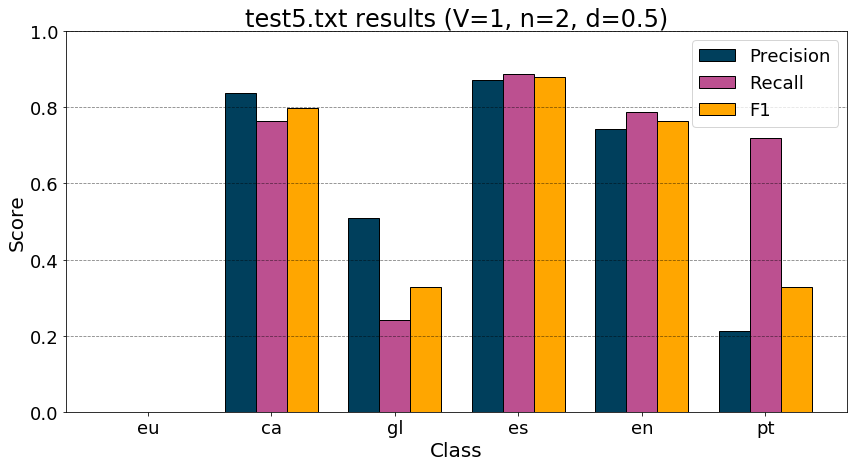
\includegraphics[width=12.5cm]{images/test5_results_1_2_0.5.png}
        \caption{Metrics on demo test set, $V=1, n=2, \delta=0.5$}
        \label{fig:demo_1_2_0.5}
    \end{center}
\end{figure}

Although the metrics improved significantly, the model still fails to perform well on the Galician and Portuguese tweets. Again, the low recall on the gl class can be explained by a larger number of observations in the test set. Conversely, the low precision on the pt class can be explained by a smaller number of observations.

\begin{table}
	\centering
	\caption{Cross tabulation of predictions, $V=1, n=2, \delta=0.5$}
	\label{tab:demo_confusion_1_2_0.5}
	\begin{tabular}{|c|c|c|c|c|c|c|c|} \hline
	    & & \multicolumn{6}{c|}{Predicted} \\ \hline
		& &    ca &   en &    es &  eu &   gl &   pt \\ \hline
		\multirow{6}{*}{Actual} & ca   &  1064 &   23 &   256 &   7 &    9 &   32 \\
		& en   &    34 &  380 &    59 &   2 &    0 &    8 \\
		& es   &   150 &   99 &  4072 &  32 &  107 &  129 \\
		& gl   &    19 &    9 &   266 &   4 &  122 &   86 \\
		& pt   &     4 &    1 &    19 &   1 &    2 &   69 \\ \hline
	\end{tabular}
\end{table}

The use of bigrams over unigrams does help however on the other classes, making this a better model.

\subsubsection{Model 3 ($V=1, n=3, \delta=1$): }
The third model had an accuracy of 0.84, a macro F1 of 0.518 and a weighted F1 of 0.811 on the demo test set. The per-class metrics are shown in Figure~\ref{fig:demo_1_3_1}.

\begin{figure}
    \begin{center}
        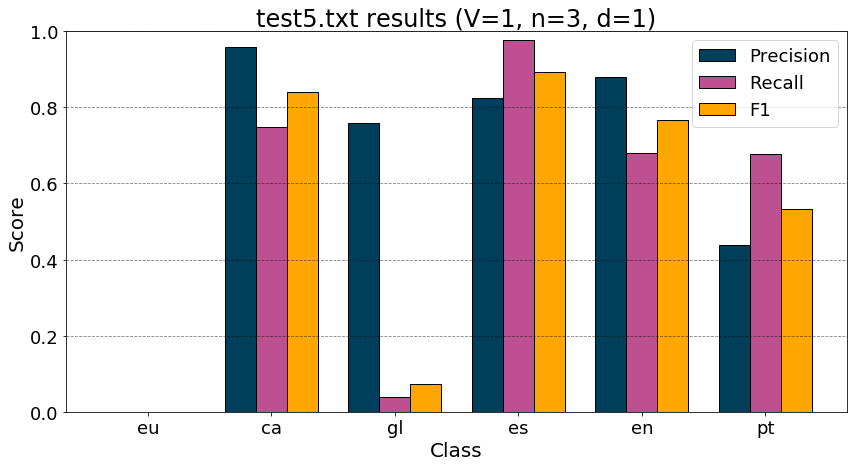
\includegraphics[width=12.5cm]{images/test5_results_1_3_1.png}
        \caption{Metrics on demo test set, $V=1, n=3, \delta=1$}
        \label{fig:demo_1_3_1}
    \end{center}
\end{figure}

Once again the metrics on this iteration of the classifier improved, most likely due to the use of trigrams. However, the recall metric on Galician tweets has further decreased while the precision has increased, indicating an under-prediction. In fact, looking at Table~\ref{tab:demo_confusion_1_3_1} shows that most false negatives of Galician tweets were classified as Spanish. However, the decrease in performance on the gl class improved the model's performance on all other classes, as their F1 scores all increased.

\begin{table}
	\centering
	\caption{Cross tabulation of predictions, $V=1, n=3, \delta=1$}
	\label{tab:demo_confusion_1_3_1}
	\begin{tabular}{|c|c|c|c|c|c|c|c|} \hline
	    & & \multicolumn{6}{c|}{Predicted} \\ \hline
		& &    ca &   en &    es &  eu &  gl &  pt \\ \hline
		\multirow{6}{*}{Actual} & ca   &  1041 &    4 &   338 &   0 &   0 &   8 \\
		& en   &    21 &  329 &   131 &   0 &   0 &   2 \\
		& es   &    20 &   40 &  4480 &   1 &   6 &  42 \\
		& gl   &     3 &    1 &   452 &   0 &  19 &  31 \\
		& pt   &     2 &    0 &    29 &   0 &   0 &  65 \\ \hline
	\end{tabular}
\end{table}

In the original test set, we observed that the trigram model (model 3) performed the best on the underrepresented class. Although this model produces the highest precision on the pt class out of all models, it doesn't produce the highest recall. However, the F1 score for Portuguese tweets does achieve a maximum under model 3.

\subsubsection{Model 4 ($V=2, n=2, \delta=0.3$): }
The fourth model had an accuracy of 0.834, a macro F1 of 0.544 and a weighted F1 of 0.826 on the demo test set. The per-class metrics are shown in Figure~\ref{fig:demo_2_2_0.3}.

\begin{figure}
    \begin{center}
        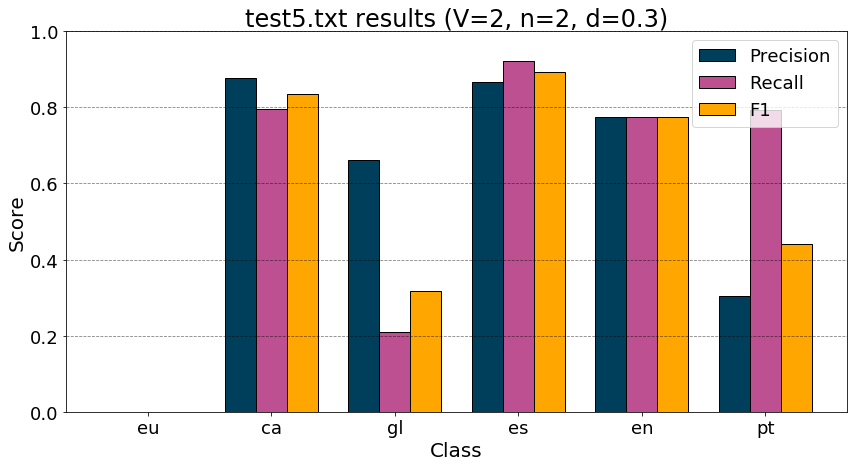
\includegraphics[width=12.5cm]{images/test5_results_2_2_0.3.png}
        \caption{Metrics on demo test set, $V=2, n=2, \delta=0.3$}
        \label{fig:demo_2_2_0.3}
    \end{center}
\end{figure}

Once again the final model produces the highest test metrics, although the accuracy only increases slightly. In addition, its performance still isn't as good as on the original test set. A look at the per-class metrics shows that the F1 score increased on Galician tweets but decreased on the Portuguese tweets, showing the re-balancing between the two classes. 

\begin{table}
	\centering
	\caption{Cross tabulation of predictions, $V=2, n=2, \delta=0.3$}
	\label{tab:demo_confusion_2_2_0.3}
	\begin{tabular}{|c|c|c|c|c|c|c|c|} \hline
	    & & \multicolumn{6}{c|}{Predicted} \\ \hline
		& &    ca &   en &    es &  eu &   gl &  pt \\ \hline
		\multirow{6}{*}{Actual} & ca   &  1107 &   18 &   239 &   7 &    2 &  18 \\
		& en   &    29 &  374 &    72 &   1 &    0 &   7 \\
		& es   &   114 &   84 &  4227 &  20 &   52 &  92 \\
		& gl   &    11 &    6 &   326 &   1 &  106 &  56 \\
		& pt   &     1 &    0 &    18 &   1 &    0 &  76 \\ \hline
	\end{tabular}
\end{table}

Other than that, the results seem similar to those of model 3. It is difficult to say whether or not the use of vocabulary 2 had a massive effect on the performance of the model, since model 3 seemed to have performed respectably on the original test set.

\begin{figure}
    \begin{center}
        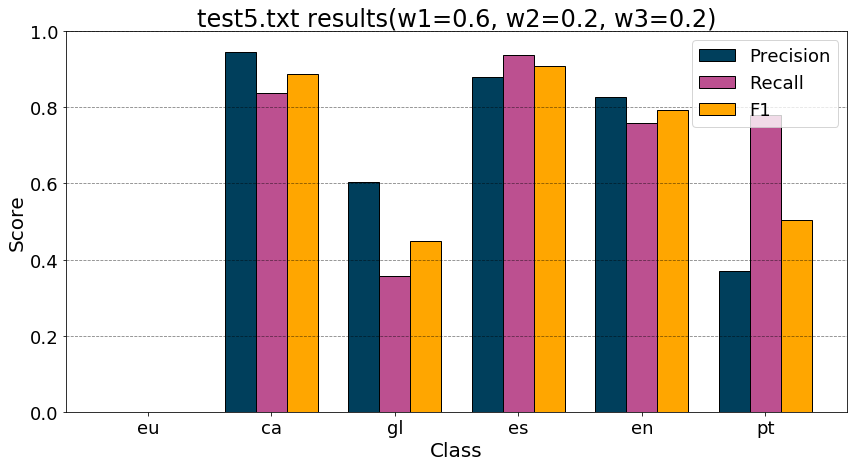
\includegraphics[width=12.5cm]{images/test5_results_BYOM.png}
        \caption{Metrics on original test set, BYOM $w_1=0.6$, $w_2=0.2$, $w_3=0.2$}
        \label{fig:demo_BYOM}
    \end{center}
\end{figure}

\newpage

\textcolor{red}{Check in appendix for all necessary confusion matrices}

\section{Team Responsibilities}

The breakdown of tasks were as follows:

\begin{enumerate}
    \item Matteo Esposito
    \begin{itemize}
        \item Project structure
        \item NBClassifier \& Ngram class
        \item utility functions \code{utils.py}
    \end{itemize}
    \item Matthew Liu
    \begin{itemize}
        \item NBClassifier \& Ngram class
        \item utility functions \code{utils.py}
    \end{itemize}
    \item Kabir Soni
    \begin{itemize}
        \item Personalized model (BYOM)
    \end{itemize}
\end{enumerate}

\begin{thebibliography}{8}
    
\bibitem{ref_2}
S.J. Russel, P. Norvig: Artificial Intelligence: A Modern Approach. 3rd edn. Pearson, Harlow (1994)

\end{thebibliography}

\section{Appendices}
\subsection{Appendix A - Confusion Matrices (Given Test Dataset \code{test-tweets-given.txt})}










\begin{table}
	\centering
	\caption{Cross tabulation of predictions (BYOM), $V=1, n=2, \delta=0.5$}
	\begin{tabular}{|c|c|c|c|c|c|c|c|} \hline
		& & \multicolumn{6}{c|}{Predicted} \\ \hline
		& &  ca &   en &    es &   eu &  gl &    pt \\ \hline
		\multirow{6}{*}{Actual} & ca   &  51 &    1 &    23 &    0 &   0 &     0 \\
		& en   &   3 &  406 &   102 &    2 &   0 &     3 \\
		& es   &  11 &   16 &  3914 &    7 &   0 &    25 \\
		& eu   &   2 &    4 &   109 &  264 &   0 &     1 \\
		& gl   &   0 &    0 &     1 &    0 &   0 &     0 \\
		& pt   &  17 &    9 &   412 &    0 &   2 &  1615 \\ \hline
	\end{tabular}
\end{table}

\newpage

\subsection{Appendix B - Confusion Matrices (Demo Dataset \code{test5.txt})}









\begin{table}
	\centering
	\caption{Cross tabulation of predictions (BYOM), $V=1, n=2, \delta=0.5$}
		\begin{tabular}{|c|c|c|c|c|c|c|c|} \hline
		& & \multicolumn{6}{c|}{Predicted} \\ \hline
		& &  ca &   en &    es &  eu &  gl &  pt \\ \hline
		\multirow{6}{*}{Actual} & ca   &  1071 &    7 &   305 &   0 &   0 &   8 \\
		& en   &    22 &  342 &   116 &   0 &   0 &   3 \\
		& es   &    19 &   44 &  4465 &   1 &  13 &  47 \\
		& gl   &     4 &    2 &   415 &   0 &  42 &  43 \\
		& pt   &     2 &    0 &    25 &   0 &   0 &  69 \\ \hline
    \end{tabular}
\end{table}

\subsection{Appendix C - Miscellaneous Code}

\subsubsection{Confusion Matrix}

\begin{lstlisting}[breaklines]
import pandas as pd

# Go through all the trace files generated during the demo.
for file in ['trace_0_1_0.txt', 'trace_1_2_0.5.txt', 'trace_1_3_1.txt', 'trace_2_2_0.3.txt', 'trace_1_BYOM_0.5.txt']:
    df = pd.read_csv(f'total_out/{file}', delimiter="  ", names=('id','lang','prob','pred_lang','res'))
    print(pd.crosstab(df['lang'], df['pred_lang']).to_latex())
\end{lstlisting}

\subsubsection{Distribution Plot}


\begin{lstlisting}[breaklines, language=Python]
import seaborn as sns
import pandas as pd
import matplotlib.pyplot as plt

orig_test = pd.read_csv(f'input/test-tweets-given.txt', delimiter="\t", names=('id','user','lang','tweet'))
demo_test = pd.read_csv(f'input/test5.txt', delimiter="\t", names=('id','user','lang','tweet'))

fig, ax = plt.subplots(figsize=(10,6))

# Cap data at tweet length of 150 and create individual plots.
orig_test['tlen'] = orig_test['tweet'].apply(len)
orig_test['tlen_capped'] = np.where(orig_test['tlen'] > 150, 150, orig_test['tlen'])
sns.distplot(orig_test.tlen_capped, ax=ax, label="Original Test Data")

demo_test['tlen'] = demo_test['tweet'].apply(len)
demo_test['tlen_capped'] = np.where(demo_test['tlen'] > 150, 150, demo_test['tlen'])
sns.distplot(demo_test.tlen_capped, ax=ax, label="Demo Test Data")

# Settings
plt.xlim(0, 150)
plt.title('test-tweets-given.txt vs. test5.txt Tweet Length Distribution')
plt.xlabel('Capped Tweet Length')
plt.legend(prop={'size': 12})
plt.ylabel('Density')
\end{lstlisting}

\end{document}

